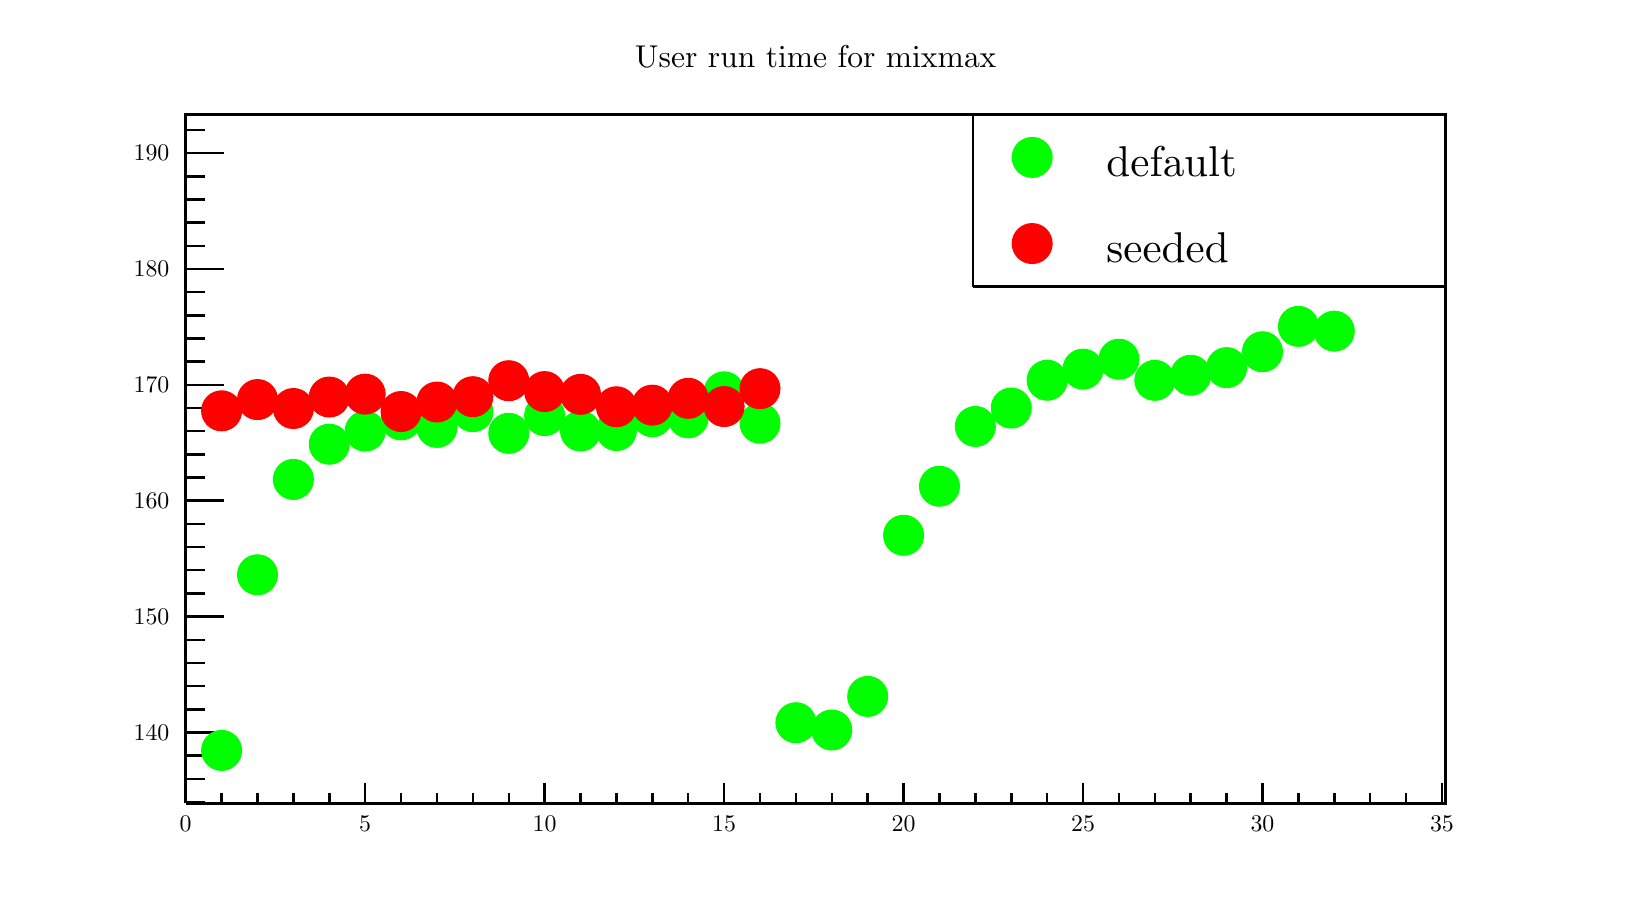
\begin{tikzpicture}
\pgfdeclareplotmark{cross} {
\pgfpathmoveto{\pgfpoint{-0.3\pgfplotmarksize}{\pgfplotmarksize}}
\pgfpathlineto{\pgfpoint{+0.3\pgfplotmarksize}{\pgfplotmarksize}}
\pgfpathlineto{\pgfpoint{+0.3\pgfplotmarksize}{0.3\pgfplotmarksize}}
\pgfpathlineto{\pgfpoint{+1\pgfplotmarksize}{0.3\pgfplotmarksize}}
\pgfpathlineto{\pgfpoint{+1\pgfplotmarksize}{-0.3\pgfplotmarksize}}
\pgfpathlineto{\pgfpoint{+0.3\pgfplotmarksize}{-0.3\pgfplotmarksize}}
\pgfpathlineto{\pgfpoint{+0.3\pgfplotmarksize}{-1.\pgfplotmarksize}}
\pgfpathlineto{\pgfpoint{-0.3\pgfplotmarksize}{-1.\pgfplotmarksize}}
\pgfpathlineto{\pgfpoint{-0.3\pgfplotmarksize}{-0.3\pgfplotmarksize}}
\pgfpathlineto{\pgfpoint{-1.\pgfplotmarksize}{-0.3\pgfplotmarksize}}
\pgfpathlineto{\pgfpoint{-1.\pgfplotmarksize}{0.3\pgfplotmarksize}}
\pgfpathlineto{\pgfpoint{-0.3\pgfplotmarksize}{0.3\pgfplotmarksize}}
\pgfpathclose
\pgfusepathqstroke
}
\pgfdeclareplotmark{cross*} {
\pgfpathmoveto{\pgfpoint{-0.3\pgfplotmarksize}{\pgfplotmarksize}}
\pgfpathlineto{\pgfpoint{+0.3\pgfplotmarksize}{\pgfplotmarksize}}
\pgfpathlineto{\pgfpoint{+0.3\pgfplotmarksize}{0.3\pgfplotmarksize}}
\pgfpathlineto{\pgfpoint{+1\pgfplotmarksize}{0.3\pgfplotmarksize}}
\pgfpathlineto{\pgfpoint{+1\pgfplotmarksize}{-0.3\pgfplotmarksize}}
\pgfpathlineto{\pgfpoint{+0.3\pgfplotmarksize}{-0.3\pgfplotmarksize}}
\pgfpathlineto{\pgfpoint{+0.3\pgfplotmarksize}{-1.\pgfplotmarksize}}
\pgfpathlineto{\pgfpoint{-0.3\pgfplotmarksize}{-1.\pgfplotmarksize}}
\pgfpathlineto{\pgfpoint{-0.3\pgfplotmarksize}{-0.3\pgfplotmarksize}}
\pgfpathlineto{\pgfpoint{-1.\pgfplotmarksize}{-0.3\pgfplotmarksize}}
\pgfpathlineto{\pgfpoint{-1.\pgfplotmarksize}{0.3\pgfplotmarksize}}
\pgfpathlineto{\pgfpoint{-0.3\pgfplotmarksize}{0.3\pgfplotmarksize}}
\pgfpathclose
\pgfusepathqfillstroke
}
\pgfdeclareplotmark{newstar} {
\pgfpathmoveto{\pgfqpoint{0pt}{\pgfplotmarksize}}
\pgfpathlineto{\pgfqpointpolar{44}{0.5\pgfplotmarksize}}
\pgfpathlineto{\pgfqpointpolar{18}{\pgfplotmarksize}}
\pgfpathlineto{\pgfqpointpolar{-20}{0.5\pgfplotmarksize}}
\pgfpathlineto{\pgfqpointpolar{-54}{\pgfplotmarksize}}
\pgfpathlineto{\pgfqpointpolar{-90}{0.5\pgfplotmarksize}}
\pgfpathlineto{\pgfqpointpolar{234}{\pgfplotmarksize}}
\pgfpathlineto{\pgfqpointpolar{198}{0.5\pgfplotmarksize}}
\pgfpathlineto{\pgfqpointpolar{162}{\pgfplotmarksize}}
\pgfpathlineto{\pgfqpointpolar{134}{0.5\pgfplotmarksize}}
\pgfpathclose
\pgfusepathqstroke
}
\pgfdeclareplotmark{newstar*} {
\pgfpathmoveto{\pgfqpoint{0pt}{\pgfplotmarksize}}
\pgfpathlineto{\pgfqpointpolar{44}{0.5\pgfplotmarksize}}
\pgfpathlineto{\pgfqpointpolar{18}{\pgfplotmarksize}}
\pgfpathlineto{\pgfqpointpolar{-20}{0.5\pgfplotmarksize}}
\pgfpathlineto{\pgfqpointpolar{-54}{\pgfplotmarksize}}
\pgfpathlineto{\pgfqpointpolar{-90}{0.5\pgfplotmarksize}}
\pgfpathlineto{\pgfqpointpolar{234}{\pgfplotmarksize}}
\pgfpathlineto{\pgfqpointpolar{198}{0.5\pgfplotmarksize}}
\pgfpathlineto{\pgfqpointpolar{162}{\pgfplotmarksize}}
\pgfpathlineto{\pgfqpointpolar{134}{0.5\pgfplotmarksize}}
\pgfpathclose
\pgfusepathqfillstroke
}
\definecolor{c}{rgb}{1,1,1};
\draw [color=c, fill=c] (0,0) rectangle (20,10.9387);
\draw [color=c, fill=c] (2,1.09387) rectangle (18,9.84481);
\definecolor{c}{rgb}{0,0,0};
\draw [c,line width=0.9] (2,1.09387) -- (2,9.84481) -- (18,9.84481) -- (18,1.09387) -- (2,1.09387);
\definecolor{c}{rgb}{1,1,1};
\draw [color=c, fill=c] (2,1.09387) rectangle (18,9.84481);
\definecolor{c}{rgb}{0,0,0};
\draw [c,line width=0.9] (2,1.09387) -- (2,9.84481) -- (18,9.84481) -- (18,1.09387) -- (2,1.09387);
\draw [c,line width=0.9] (2,1.09387) -- (18,1.09387);
\draw [c,line width=0.9] (2,1.3564) -- (2,1.09387);
\draw [c,line width=0.9] (2.45584,1.22513) -- (2.45584,1.09387);
\draw [c,line width=0.9] (2.91168,1.22513) -- (2.91168,1.09387);
\draw [c,line width=0.9] (3.36752,1.22513) -- (3.36752,1.09387);
\draw [c,line width=0.9] (3.82336,1.22513) -- (3.82336,1.09387);
\draw [c,line width=0.9] (4.2792,1.3564) -- (4.2792,1.09387);
\draw [c,line width=0.9] (4.73504,1.22513) -- (4.73504,1.09387);
\draw [c,line width=0.9] (5.19088,1.22513) -- (5.19088,1.09387);
\draw [c,line width=0.9] (5.64672,1.22513) -- (5.64672,1.09387);
\draw [c,line width=0.9] (6.10256,1.22513) -- (6.10256,1.09387);
\draw [c,line width=0.9] (6.5584,1.3564) -- (6.5584,1.09387);
\draw [c,line width=0.9] (7.01425,1.22513) -- (7.01425,1.09387);
\draw [c,line width=0.9] (7.47009,1.22513) -- (7.47009,1.09387);
\draw [c,line width=0.9] (7.92593,1.22513) -- (7.92593,1.09387);
\draw [c,line width=0.9] (8.38177,1.22513) -- (8.38177,1.09387);
\draw [c,line width=0.9] (8.83761,1.3564) -- (8.83761,1.09387);
\draw [c,line width=0.9] (9.29345,1.22513) -- (9.29345,1.09387);
\draw [c,line width=0.9] (9.74929,1.22513) -- (9.74929,1.09387);
\draw [c,line width=0.9] (10.2051,1.22513) -- (10.2051,1.09387);
\draw [c,line width=0.9] (10.661,1.22513) -- (10.661,1.09387);
\draw [c,line width=0.9] (11.1168,1.3564) -- (11.1168,1.09387);
\draw [c,line width=0.9] (11.5726,1.22513) -- (11.5726,1.09387);
\draw [c,line width=0.9] (12.0285,1.22513) -- (12.0285,1.09387);
\draw [c,line width=0.9] (12.4843,1.22513) -- (12.4843,1.09387);
\draw [c,line width=0.9] (12.9402,1.22513) -- (12.9402,1.09387);
\draw [c,line width=0.9] (13.396,1.3564) -- (13.396,1.09387);
\draw [c,line width=0.9] (13.8519,1.22513) -- (13.8519,1.09387);
\draw [c,line width=0.9] (14.3077,1.22513) -- (14.3077,1.09387);
\draw [c,line width=0.9] (14.7635,1.22513) -- (14.7635,1.09387);
\draw [c,line width=0.9] (15.2194,1.22513) -- (15.2194,1.09387);
\draw [c,line width=0.9] (15.6752,1.3564) -- (15.6752,1.09387);
\draw [c,line width=0.9] (16.1311,1.22513) -- (16.1311,1.09387);
\draw [c,line width=0.9] (16.5869,1.22513) -- (16.5869,1.09387);
\draw [c,line width=0.9] (17.0427,1.22513) -- (17.0427,1.09387);
\draw [c,line width=0.9] (17.4986,1.22513) -- (17.4986,1.09387);
\draw [c,line width=0.9] (17.9544,1.3564) -- (17.9544,1.09387);
\draw [c,line width=0.9] (17.9544,1.3564) -- (17.9544,1.09387);
\draw [anchor=base] (2,0.732891) node[scale=0.861703, color=c, rotate=0]{0};
\draw [anchor=base] (4.2792,0.732891) node[scale=0.861703, color=c, rotate=0]{5};
\draw [anchor=base] (6.5584,0.732891) node[scale=0.861703, color=c, rotate=0]{10};
\draw [anchor=base] (8.83761,0.732891) node[scale=0.861703, color=c, rotate=0]{15};
\draw [anchor=base] (11.1168,0.732891) node[scale=0.861703, color=c, rotate=0]{20};
\draw [anchor=base] (13.396,0.732891) node[scale=0.861703, color=c, rotate=0]{25};
\draw [anchor=base] (15.6752,0.732891) node[scale=0.861703, color=c, rotate=0]{30};
\draw [anchor=base] (17.9544,0.732891) node[scale=0.861703, color=c, rotate=0]{35};
\draw [c,line width=0.9] (2,1.09387) -- (2,9.84481);
\draw [c,line width=0.9] (2.48,1.99508) -- (2,1.99508);
\draw [c,line width=0.9] (2.24,2.28935) -- (2,2.28935);
\draw [c,line width=0.9] (2.24,2.58362) -- (2,2.58362);
\draw [c,line width=0.9] (2.24,2.8779) -- (2,2.8779);
\draw [c,line width=0.9] (2.24,3.17217) -- (2,3.17217);
\draw [c,line width=0.9] (2.48,3.46644) -- (2,3.46644);
\draw [c,line width=0.9] (2.24,3.76072) -- (2,3.76072);
\draw [c,line width=0.9] (2.24,4.05499) -- (2,4.05499);
\draw [c,line width=0.9] (2.24,4.34926) -- (2,4.34926);
\draw [c,line width=0.9] (2.24,4.64353) -- (2,4.64353);
\draw [c,line width=0.9] (2.48,4.93781) -- (2,4.93781);
\draw [c,line width=0.9] (2.24,5.23208) -- (2,5.23208);
\draw [c,line width=0.9] (2.24,5.52635) -- (2,5.52635);
\draw [c,line width=0.9] (2.24,5.82062) -- (2,5.82062);
\draw [c,line width=0.9] (2.24,6.1149) -- (2,6.1149);
\draw [c,line width=0.9] (2.48,6.40917) -- (2,6.40917);
\draw [c,line width=0.9] (2.24,6.70344) -- (2,6.70344);
\draw [c,line width=0.9] (2.24,6.99772) -- (2,6.99772);
\draw [c,line width=0.9] (2.24,7.29199) -- (2,7.29199);
\draw [c,line width=0.9] (2.24,7.58626) -- (2,7.58626);
\draw [c,line width=0.9] (2.48,7.88053) -- (2,7.88053);
\draw [c,line width=0.9] (2.24,8.17481) -- (2,8.17481);
\draw [c,line width=0.9] (2.24,8.46908) -- (2,8.46908);
\draw [c,line width=0.9] (2.24,8.76335) -- (2,8.76335);
\draw [c,line width=0.9] (2.24,9.05763) -- (2,9.05763);
\draw [c,line width=0.9] (2.48,9.3519) -- (2,9.3519);
\draw [c,line width=0.9] (2.48,1.99508) -- (2,1.99508);
\draw [c,line width=0.9] (2.24,1.70081) -- (2,1.70081);
\draw [c,line width=0.9] (2.24,1.40653) -- (2,1.40653);
\draw [c,line width=0.9] (2.24,1.11226) -- (2,1.11226);
\draw [c,line width=0.9] (2.48,9.3519) -- (2,9.3519);
\draw [c,line width=0.9] (2.24,9.64617) -- (2,9.64617);
\draw [anchor= east] (1.9,1.99508) node[scale=0.861703, color=c, rotate=0]{140};
\draw [anchor= east] (1.9,3.46644) node[scale=0.861703, color=c, rotate=0]{150};
\draw [anchor= east] (1.9,4.93781) node[scale=0.861703, color=c, rotate=0]{160};
\draw [anchor= east] (1.9,6.40917) node[scale=0.861703, color=c, rotate=0]{170};
\draw [anchor= east] (1.9,7.88053) node[scale=0.861703, color=c, rotate=0]{180};
\draw [anchor= east] (1.9,9.3519) node[scale=0.861703, color=c, rotate=0]{190};
\definecolor{c}{rgb}{0,1,0};
\foreach \P in {(2.45584,1.76702), (2.91168,3.9976), (3.36752,5.20854), (3.82336,5.65583), (4.2792,5.8221), (4.73504,5.96482), (5.19088,5.86918), (5.64672,6.06929), (6.10256,5.79414), (6.5584,6.01926), (7.01425,5.82357), (7.47009,5.82945),
 (7.92593,6.00455), (8.38177,5.9913), (8.83761,6.32089), (9.29345,5.92215), (9.74929,2.11867), (10.2051,2.02598), (10.661,2.45267), (11.1168,4.49934), (11.5726,5.12173), (12.0285,5.88095), (12.4843,6.1149), (12.9402,6.46802), (13.396,6.60928),
 (13.8519,6.73434), (14.3077,6.46655), (14.7635,6.53129), (15.2194,6.6284), (15.6752,6.82998), (16.1311,7.15221), (16.5869,7.09188)}{\draw[mark options={color=c,fill=c},mark size=7.207207pt,mark=*] plot coordinates {\P};}
\definecolor{c}{rgb}{1,0,0};
\foreach \P in {(2.45584,6.07958), (2.91168,6.22231), (3.36752,6.10901), (3.82336,6.25468), (4.2792,6.29146), (4.73504,6.07076), (5.19088,6.19141), (5.64672,6.25909), (6.10256,6.46214), (6.5584,6.32383), (7.01425,6.28852), (7.47009,6.13108),
 (7.92593,6.15168), (8.38177,6.23849), (8.83761,6.13403), (9.29345,6.36062)}{\draw[mark options={color=c,fill=c},mark size=7.207207pt,mark=*] plot coordinates {\P};}
\definecolor{c}{rgb}{1,1,1};
\draw [color=c, fill=c] (12,7.65707) rectangle (18,9.84481);
\definecolor{c}{rgb}{0,0,0};
\draw [c,line width=0.9] (12,7.65707) -- (18,7.65707);
\draw [c,line width=0.9] (18,7.65707) -- (18,9.84481);
\draw [c,line width=0.9] (18,9.84481) -- (12,9.84481);
\draw [c,line width=0.9] (12,9.84481) -- (12,7.65707);
\draw [anchor=base west] (13.5,9.05175) node[scale=1.55662, color=c, rotate=0]{default};
\definecolor{c}{rgb}{1,1,1};
\draw [c] (12.225,8.91502) -- (13.275,8.91502) -- (13.275,9.68073) -- (12.225,9.68073);
\draw [c,line width=0.9] (12.225,9.29787) -- (13.275,9.29787);
\definecolor{c}{rgb}{0,1,0};
\foreach \P in {(12.75,9.29787)}{\draw[mark options={color=c,fill=c},mark size=7.207207pt,mark=*] plot coordinates {\P};}
\definecolor{c}{rgb}{0,0,0};
\draw [anchor=base west] (13.5,7.95788) node[scale=1.55662, color=c, rotate=0]{seeded};
\definecolor{c}{rgb}{1,1,1};
\draw [c] (12.225,7.82115) -- (13.275,7.82115) -- (13.275,8.58686) -- (12.225,8.58686);
\draw [c,line width=0.9] (12.225,8.204) -- (13.275,8.204);
\definecolor{c}{rgb}{1,0,0};
\foreach \P in {(12.75,8.204)}{\draw[mark options={color=c,fill=c},mark size=7.207207pt,mark=*] plot coordinates {\P};}
\definecolor{c}{rgb}{0,0,0};
\draw (10,10.5832) node[scale=1.13967, color=c, rotate=0]{User run time for mixmax};
\end{tikzpicture}
